\documentclass[tikz,11pt]{standalone}

% --- Packages ---
\usepackage{amsmath,amssymb}
\usepackage[scaled]{helvet}
\usepackage{transfer_matrix}
\renewcommand\familydefault{\sfdefault}
\usetikzlibrary{arrows.meta, positioning, fit, matrix, patterns,intersections}

% --- Parameters ---
\newcommand{\pS}{5}
\newcommand{\timeStep}{4}
\newcommand{\lookAheadHours}{8}
\newcommand{\controlHours}{4}
\newcommand{\noIterations}{5}

% --- Styles ---
\tikzset{
  horizon/.style={draw=black, line width=0.4pt, minimum height=\pS*\unit},
  lookahead/.style={horizon, pattern=north west lines, pattern color=black},
  control/.style={horizon, pattern=north east lines, pattern color=gray!70!black, dashed},
  arrowLine/.style={line width=0.5pt, -{Triangle[length=2mm,width=2mm]}},
  tick/.style={line width=0.4pt},
  textNode/.style={font=\scriptsize, inner sep=1pt}
}

\begin{document}
\begin{tikzpicture}[x=\unit,y=\unit]

% --- Draw horizons (lookahead + control) ---
\foreach \i in {0,...,\numexpr\noIterations-1} {
  \pgfmathsetmacro{\x}{\i*\timeStep*\pS}
  \pgfmathsetmacro{\y}{-\i*\timeStep*\pS}

  % Lookahead band
  \draw[lookahead] (\x,\y-\pS) rectangle ++(\lookAheadHours*\pS,\pS);

  % Control band
  \draw[control] (\x,\y-2.5*\pS) rectangle ++(\controlHours*\pS,\pS);
}

% --- Time axis + ticks ---
\pgfmathsetmacro{\axisLength}{\noIterations*\timeStep*\pS + (\lookAheadHours*\pS)/1.5}
\pgfmathsetmacro{\axisY}{-(\noIterations)*\timeStep*\pS}

% Draw axis line
\draw[arrowLine] (0,\axisY) -- (\axisLength,\axisY) node[right]{\scriptsize Time};

% Axis ticks with labels
\pgfmathtruncatemacro{\lastTick}{\noIterations*\timeStep + \lookAheadHours}
\pgfmathtruncatemacro{\nTicks}{(\lastTick/\timeStep)-1}
\foreach \n in {0,...,\nTicks} {
	\pgfmathsetmacro{\xtick}{\n * \timeStep * \pS}
	\pgfmathtruncatemacro{\ticklabel}{\n * \timeStep}
	\draw (\xtick*\unit,\axisY*\unit-0.5*\pS*\unit) -- ++(0,3);
	\node[textNode] at (\xtick*\unit,\axisY*\unit-1.5*\pS*\unit) {\ticklabel}; 
}

% --- Magnified transfer matrix ---
\pgfmathsetmacro{\lastX}{(\noIterations-1)*\timeStep*\pS}
\pgfmathsetmacro{\lastY}{-(\noIterations-1)*\timeStep*\pS}
\pgfmathsetmacro{\matrixX}{(\noIterations-4.5)*\timeStep*\pS}
\pgfmathsetmacro{\matrixY}{\lastY - 2*\pS}

% Insert scaled TransferMatrix
\node[anchor=south west, inner sep=0pt] (tmatrix) at (\matrixX,\matrixY) {%
  \begin{tikzpicture}[scale=0.45, transform shape]
    \TransferMatrix
  \end{tikzpicture}
};

% Circle highlight around matrix
\node[draw, circle, fit=(tmatrix), inner sep=1pt] (circ) {};

% Connection arrow from last horizon to magnified matrix
\pgfmathsetmacro{\horizonY}{\lastY - 0.5*\pS}
\draw[arrowLine, dashed] 
  (\lastX,\horizonY) -- 
  ([xshift=\pgfkeysvalueof{/pgf/outer xsep}] circ.east |- 0,\horizonY);

% --- Legend ---
\node[anchor=north east, inner sep=2pt] at (current bounding box.north east) {%
  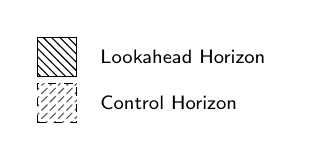
\begin{tikzpicture}
    \matrix[matrix of nodes,row sep=2pt,column sep=5pt,
            nodes={anchor=west,font=\scriptsize}] {
      \node[lookahead, minimum size=5mm] {}; & Lookahead Horizon \\
      \node[control,   minimum size=5mm] {}; & Control Horizon \\
    };
  \end{tikzpicture}
};

\end{tikzpicture}
\end{document}